\documentclass{article}

\usepackage{graphicx}
\usepackage{tikz}
\usepackage{tikzsymbols}
\usetikzlibrary{calc,patterns,shapes.geometric}
\pagestyle{empty}
\usepackage[margin=0pt]{geometry}
\geometry{papersize={14in,12in}}

\def\centerarc[#1](#2)(#3:#4:#5){\draw[#1] ($(#2)+({#5*cos(#3)},{#5*sin(#3)})$) arc (#3:#4:#5);}

\begin{document}
	\begin{figure}
		\centering
		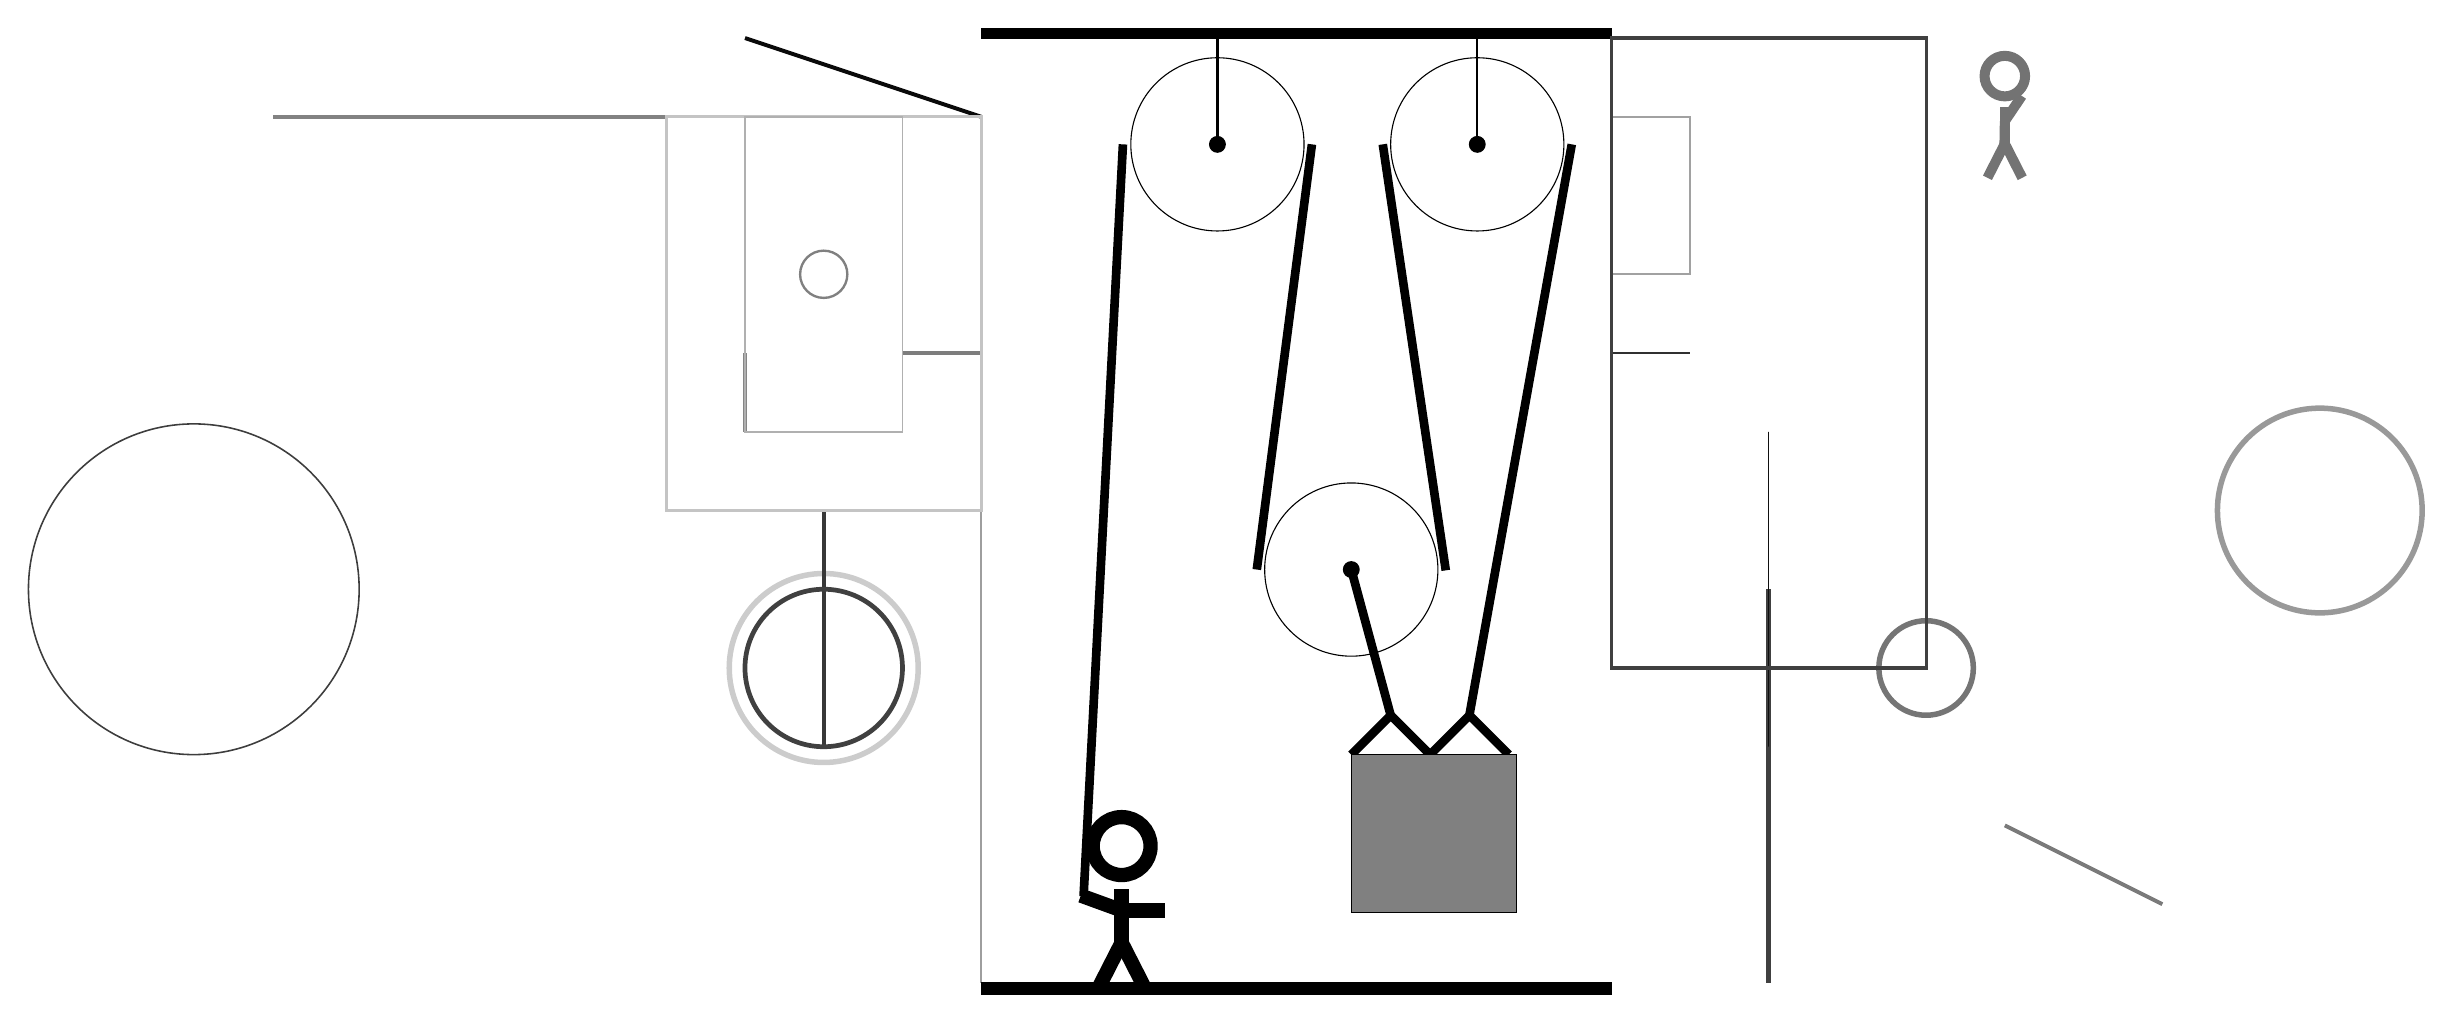
\begin{tikzpicture}
			%%%%% START %%%%%
			
			\draw[fill=black] (-2, 9) rectangle (6, 9.125);
			
			\draw (1, 7.65) circle (1.1);
			\draw[fill=black] (1, 7.65) circle (0.1);
			\draw[thick] (1, 7.65) -- (1, 9);
			
			\draw (4.3, 7.65) circle (1.1);
			\draw[fill=black] (4.3, 7.65) circle (0.1);
			\draw[thick] (4.3, 7.65) -- (4.3, 9);
			
			\draw (2.7, 2.25) circle (1.1);
			\draw[fill=black] (2.7, 2.25) circle (0.1);
			
			\draw[line width=1.1mm]  (2.7, -0.1) -- (3.2, 0.4) -- (3.7, -0.1) -- (4.2, 0.4) -- (4.7, -0.1);
			\draw[fill=black!50] (2.7, -0.1) rectangle (4.8, -2.1);
			
			\draw[line width=1.1mm](-0.7, -1.9) -- (-0.2, 7.65);
			\centerarc[line width=1.1mm](1, 7.65)(0:180:1.2000000000000002);
			\draw[line width=1.1mm](2.2, 7.65) -- (1.5, 2.25);
			\centerarc[line width=1.1mm](2.7, 2.25)(180:370:1.2000000000000002);
			\draw[line width=1.1mm] (3.9, 2.24) -- (3.1, 7.65);
			\centerarc[line width=1.1mm](4.3, 7.65)(0:180:1.2000000000000002);
			\draw[line width=1.1mm](4.2, 0.4) -- (5.5, 7.65);
			\draw[line width=1.1mm] (3.2, 0.4) -- (2.7, 2.25);
			
			\node at (-0.2, -2) {\Strichmaxerl[10][-20][0]};
			
			\draw[line width=0.4mm, color=black!51] (-3, 5) rectangle (-2, 5);
			
			\draw [line width=0.7mm, color=black!20](-4, 1) circle (1.2);
			\draw[line width=0.5mm, color=black!49](-6, 8) -- (-11, 8);
			\draw[line width=0.5mm, color=black!52](11, -1) -- (13, -2);
			\draw [line width=0.7mm, color=black!40](15, 3) circle (1.3);
			\draw[line width=0.5mm, color=black!96](-5, 9) -- (-2, 8);
			
			\draw[line width=0.3mm, color=black!81] (7, 5) rectangle (6, 5);
			\draw [line width=0.7mm, color=black!54](10, 1) circle (0.6);
			\draw[line width=0.5mm, color=black!78](-4, 3) -- (-4, 0);
			
			\draw[line width=0.6mm, color=black!75] (8, -3) rectangle (8, 2);
			\draw[line width=0.5mm, color=black!48](-5, 5) -- (-5, 4);
			\draw[line width=0.2mm, color=black!94] (8, 4) rectangle (8, 0);
			\draw[line width=0.3mm, color=black!37] (6, 8) rectangle (7, 6);
			
			\draw [line width=0.3mm, color=black!50](-4, 6) circle (0.3);
			\node[line width=0.7mm, color=black!55] at (11, 8) {\Strichmaxerl[7][89][56]};
			\draw[line width=0.3mm, color=black!38] (-2, -3) rectangle (-2, 3);
			
			\draw[line width=0.4mm, color=black!75] (6, 9) rectangle (10, 1);
			
			\draw [line width=0.2mm, color=black!76](-12, 2) circle (2.1);
			\draw[line width=0.4mm, color=black!23] (-2, 8) rectangle (-6, 3);
			
			\draw[line width=0.2mm, color=black!31] (-3, 8) rectangle (-5, 4);
			\draw [line width=0.6mm, color=black!75](-4, 1) circle (1.0);
			
			\draw[fill=black] (-2, -3) rectangle (6, -3.15);
			
			%%%%% END %%%%%
		\end{tikzpicture}
	\end{figure}	
\end{document}